\documentclass[10pt]{article}
\usepackage{pgfplots}
\pgfplotsset{compat=1.15}
\usepackage{mathrsfs}
\usetikzlibrary{arrows}
\pagestyle{empty}
\begin{document}
\definecolor{qqqqff}{rgb}{0.,0.,1.}
\definecolor{zzttqq}{rgb}{0.6,0.2,0.}
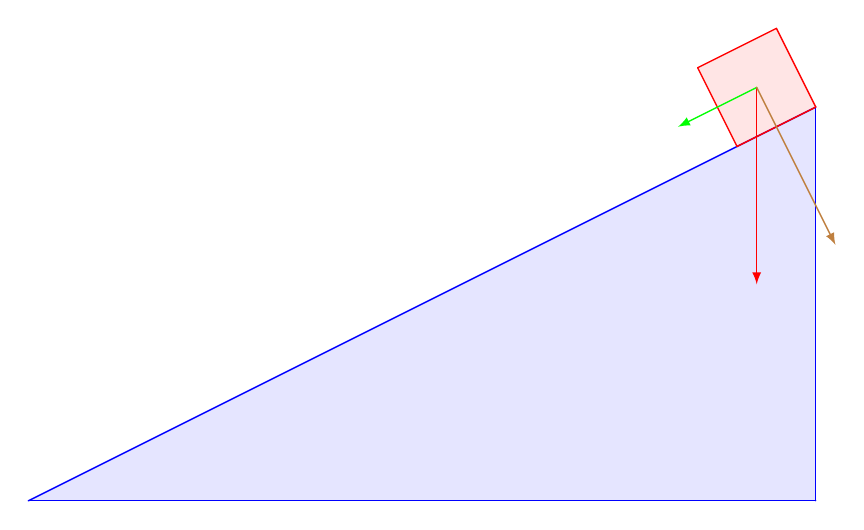
\begin{tikzpicture}[line cap=round,line join=round,>=triangle 45,x=0.5cm,y=0.5cm]
\fill[line width=2.pt,color=blue,fill=blue,fill opacity=0.1] (0.,0.) -- (20.,0.) -- (20.,10.) -- cycle;
\fill[line width=2.pt,color=red,fill=red,fill opacity=0.1] (20.,10.) -- (18.,9.) -- (17.,11.) -- (19.,12.) -- cycle;
\draw [line width=0.5pt,color=blue] (0.,0.)-- (20.,0.);
\draw [line width=0.5pt,color=blue] (20.,0.)-- (20.,10.);
\draw [line width=0.5pt,color=blue] (20.,10.)-- (0.,0.);
\draw [line width=0.5pt,color=red] (20.,10.)-- (18.,9.);
\draw [line width=0.5pt,color=red] (18.,9.)-- (17.,11.);
\draw [line width=0.5pt,color=red] (17.,11.)-- (19.,12.);
\draw [line width=0.5pt,color=red] (19.,12.)-- (20.,10.);
\draw [->,>=latex,line width=0.5pt, red] (18.5,10.5) -- (18.5,5.5);
\draw [->,>=latex,line width=0.5pt, green] (18.5,10.5) -- (16.5,9.5);
\draw [->,>=latex,line width=0.5pt, brown] (18.5,10.5) -- (20.5,6.5);
\end{tikzpicture}
\end{document}